\subsubsection{Progress}

\begin{itemize}
    \item \textbf{Recurrent Neural Networks}
    
        \begin{figure}[H]
            \centering
            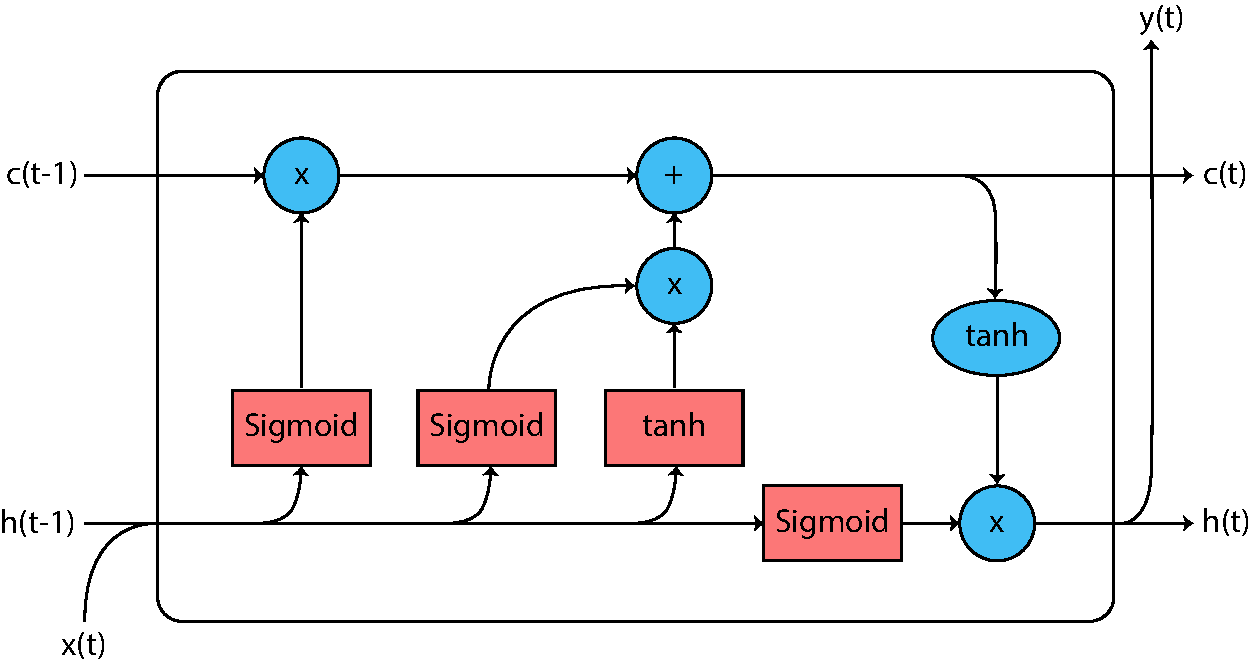
\includegraphics[width=0.75\linewidth]{resources/lstm_node.pdf}
            \caption{An individual LSTM node. The red boxes represent layers (with learnt weights and biases) with their labelled activation functions. The blue components are element-wise operations. Any place where a signal trace splits or joins, the signal is copied or added respectively.}
            \label{fig:lstm_node}
        \end{figure}
    
        Due to inter-symbol interference introduced by the chromatic dispersion in the fiber link, introducing a notion of memory for the neural network to leverage seemed like it may be beneficial at the encoding and/or decoding neural networks. Recurrent Neural Networks (RNNs) are a group of well documented neural network architectures that feature memory between consecutive time-steps. These are most commonly used in time-series data for forecasting applications. A common RNN is the Long-Short Term Memory (LSTM) node and one of it's nodes is depicted in Fig. \ref{fig:lstm_node}. These layers were implemented at the encoding and decoding neural network to introduce a notion of memory. However, when training was commenced, the neural network did not converge to a solution and produced a model with a symbol error rate equivalent to that of random guesses. An alternate configuration with the LSTM just on the decoding neural network was also implemented and this configuration was no better. \\
        \\
        Something that may be worthy of investigating and implementing are different RNN nodes such as SimpleRNN and GRU. Additionally, further investigation into the working of RNN training may be required to identify the issues I am experiencing while training with these layers.
    
    \item \textbf{Symbol to Bit mapping}
    
        The current implementation of the auto-encoder, as shown in Fig. X, learns the optimal mapping of symbols on samples. This minimizes the symbol error rate but not necessarily the bit error rate. In order to learn the most optimal mapping of bits to symbols, many different methodologies were attempted. Initially, the inputs to the neural network were modified from one-hot encoded inputs to simply a bit representation with a cost function of binary cross entropy for which the equation is given below:
        
        \begin{equation}
            L=y_{true}\log\left(y_{pred}\right) + (1-y_{true})\log\left(1-y_{pred}\right)
        \end{equation}
        
        This cost function is suited for data with 1s and 0s as in this case. This configuration of the neural network did not however converge to a solution. Furthermore, investigation into a custom loss function was also done with no success.
        
        \begin{figure}[H]
            \centering
            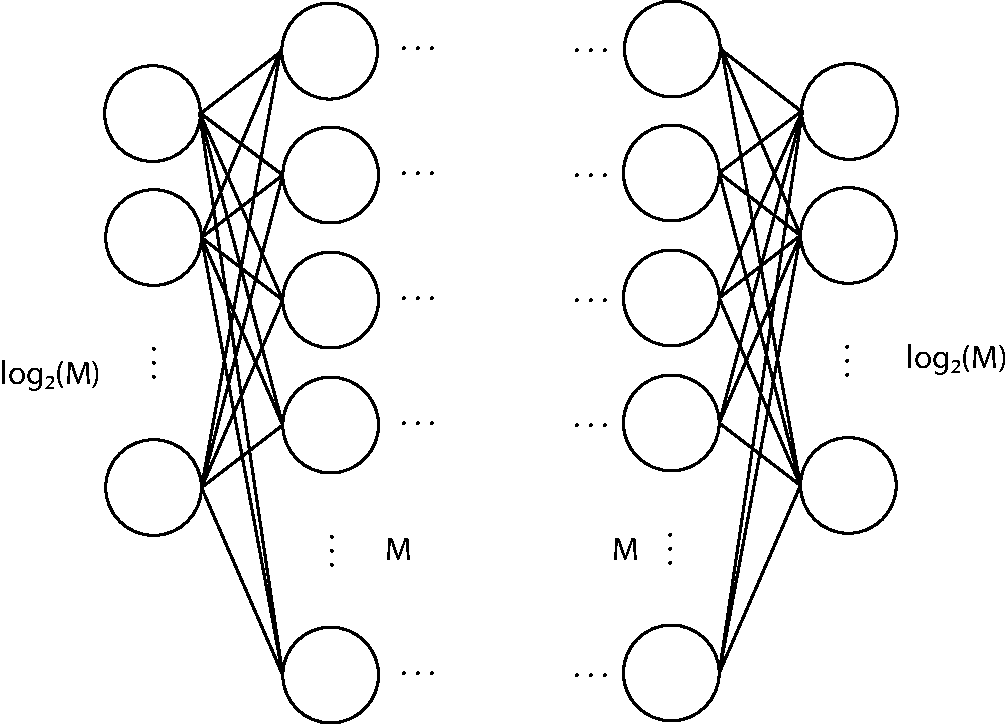
\includegraphics[width=0.75\linewidth]{resources/symbol_mapping.pdf}
            \caption{These layers convert a bit representation of the symbol to a one-hot encoded representation. For example in the case of 2 bits per symbol, $M=4$ and the bits 01 would be encoded as $(0,0,1,0)$.}
            \label{fig:symbol_mapping}
        \end{figure}
        
        Finally, I implemented layers that would convert from bit representation to a one-hot encoded symbol and the inverse as shown in Fig. \ref{fig:symbol_mapping}. These layers could be placed at the beginning and end of the existing auto-encoder.These layers may be used to iteratively learn a symbol and bit mapping. This is done by initially training the network with one-hot encoded inputs/outputs (without the layers shown in Fig. \ref{fig:symbol_mapping}). Once training has finished, a second model with the bit-symbol mapping layers is trained on bit representation of the symbols. This forces the neural network to minimize the bit error rate. This process is repeated for a pre-determined number of steps until the error converges to a minimum
    
\end{itemize}

\subsubsection{Difficulties Encountered}
    
    The main difficulty that I encountered during this period was the model not converging to a minimum loss for given configurations. To understand why this occurs I will need to further look into the fundamentals of neural networks and it's implementation in keras/tensorflow. I was not able to implement a working model with recurrent neural networks and will need to do further research into the workings of RNNs such as LSTM and SimpleRNN. The training time for some of these models are in the order of 30minutes on my personal computer but this problem was overcome but using the department provided Athens GPU server. 